% Options for packages loaded elsewhere
\PassOptionsToPackage{unicode}{hyperref}
\PassOptionsToPackage{hyphens}{url}
\PassOptionsToPackage{dvipsnames,svgnames,x11names}{xcolor}
%
\documentclass[
  letterpaper,
  DIV=11,
  numbers=noendperiod]{scrartcl}

\usepackage{amsmath,amssymb}
\usepackage{iftex}
\ifPDFTeX
  \usepackage[T1]{fontenc}
  \usepackage[utf8]{inputenc}
  \usepackage{textcomp} % provide euro and other symbols
\else % if luatex or xetex
  \usepackage{unicode-math}
  \defaultfontfeatures{Scale=MatchLowercase}
  \defaultfontfeatures[\rmfamily]{Ligatures=TeX,Scale=1}
\fi
\usepackage{lmodern}
\ifPDFTeX\else  
    % xetex/luatex font selection
\fi
% Use upquote if available, for straight quotes in verbatim environments
\IfFileExists{upquote.sty}{\usepackage{upquote}}{}
\IfFileExists{microtype.sty}{% use microtype if available
  \usepackage[]{microtype}
  \UseMicrotypeSet[protrusion]{basicmath} % disable protrusion for tt fonts
}{}
\makeatletter
\@ifundefined{KOMAClassName}{% if non-KOMA class
  \IfFileExists{parskip.sty}{%
    \usepackage{parskip}
  }{% else
    \setlength{\parindent}{0pt}
    \setlength{\parskip}{6pt plus 2pt minus 1pt}}
}{% if KOMA class
  \KOMAoptions{parskip=half}}
\makeatother
\usepackage{xcolor}
\setlength{\emergencystretch}{3em} % prevent overfull lines
\setcounter{secnumdepth}{-\maxdimen} % remove section numbering
% Make \paragraph and \subparagraph free-standing
\ifx\paragraph\undefined\else
  \let\oldparagraph\paragraph
  \renewcommand{\paragraph}[1]{\oldparagraph{#1}\mbox{}}
\fi
\ifx\subparagraph\undefined\else
  \let\oldsubparagraph\subparagraph
  \renewcommand{\subparagraph}[1]{\oldsubparagraph{#1}\mbox{}}
\fi

\usepackage{color}
\usepackage{fancyvrb}
\newcommand{\VerbBar}{|}
\newcommand{\VERB}{\Verb[commandchars=\\\{\}]}
\DefineVerbatimEnvironment{Highlighting}{Verbatim}{commandchars=\\\{\}}
% Add ',fontsize=\small' for more characters per line
\usepackage{framed}
\definecolor{shadecolor}{RGB}{241,243,245}
\newenvironment{Shaded}{\begin{snugshade}}{\end{snugshade}}
\newcommand{\AlertTok}[1]{\textcolor[rgb]{0.68,0.00,0.00}{#1}}
\newcommand{\AnnotationTok}[1]{\textcolor[rgb]{0.37,0.37,0.37}{#1}}
\newcommand{\AttributeTok}[1]{\textcolor[rgb]{0.40,0.45,0.13}{#1}}
\newcommand{\BaseNTok}[1]{\textcolor[rgb]{0.68,0.00,0.00}{#1}}
\newcommand{\BuiltInTok}[1]{\textcolor[rgb]{0.00,0.23,0.31}{#1}}
\newcommand{\CharTok}[1]{\textcolor[rgb]{0.13,0.47,0.30}{#1}}
\newcommand{\CommentTok}[1]{\textcolor[rgb]{0.37,0.37,0.37}{#1}}
\newcommand{\CommentVarTok}[1]{\textcolor[rgb]{0.37,0.37,0.37}{\textit{#1}}}
\newcommand{\ConstantTok}[1]{\textcolor[rgb]{0.56,0.35,0.01}{#1}}
\newcommand{\ControlFlowTok}[1]{\textcolor[rgb]{0.00,0.23,0.31}{#1}}
\newcommand{\DataTypeTok}[1]{\textcolor[rgb]{0.68,0.00,0.00}{#1}}
\newcommand{\DecValTok}[1]{\textcolor[rgb]{0.68,0.00,0.00}{#1}}
\newcommand{\DocumentationTok}[1]{\textcolor[rgb]{0.37,0.37,0.37}{\textit{#1}}}
\newcommand{\ErrorTok}[1]{\textcolor[rgb]{0.68,0.00,0.00}{#1}}
\newcommand{\ExtensionTok}[1]{\textcolor[rgb]{0.00,0.23,0.31}{#1}}
\newcommand{\FloatTok}[1]{\textcolor[rgb]{0.68,0.00,0.00}{#1}}
\newcommand{\FunctionTok}[1]{\textcolor[rgb]{0.28,0.35,0.67}{#1}}
\newcommand{\ImportTok}[1]{\textcolor[rgb]{0.00,0.46,0.62}{#1}}
\newcommand{\InformationTok}[1]{\textcolor[rgb]{0.37,0.37,0.37}{#1}}
\newcommand{\KeywordTok}[1]{\textcolor[rgb]{0.00,0.23,0.31}{#1}}
\newcommand{\NormalTok}[1]{\textcolor[rgb]{0.00,0.23,0.31}{#1}}
\newcommand{\OperatorTok}[1]{\textcolor[rgb]{0.37,0.37,0.37}{#1}}
\newcommand{\OtherTok}[1]{\textcolor[rgb]{0.00,0.23,0.31}{#1}}
\newcommand{\PreprocessorTok}[1]{\textcolor[rgb]{0.68,0.00,0.00}{#1}}
\newcommand{\RegionMarkerTok}[1]{\textcolor[rgb]{0.00,0.23,0.31}{#1}}
\newcommand{\SpecialCharTok}[1]{\textcolor[rgb]{0.37,0.37,0.37}{#1}}
\newcommand{\SpecialStringTok}[1]{\textcolor[rgb]{0.13,0.47,0.30}{#1}}
\newcommand{\StringTok}[1]{\textcolor[rgb]{0.13,0.47,0.30}{#1}}
\newcommand{\VariableTok}[1]{\textcolor[rgb]{0.07,0.07,0.07}{#1}}
\newcommand{\VerbatimStringTok}[1]{\textcolor[rgb]{0.13,0.47,0.30}{#1}}
\newcommand{\WarningTok}[1]{\textcolor[rgb]{0.37,0.37,0.37}{\textit{#1}}}

\providecommand{\tightlist}{%
  \setlength{\itemsep}{0pt}\setlength{\parskip}{0pt}}\usepackage{longtable,booktabs,array}
\usepackage{calc} % for calculating minipage widths
% Correct order of tables after \paragraph or \subparagraph
\usepackage{etoolbox}
\makeatletter
\patchcmd\longtable{\par}{\if@noskipsec\mbox{}\fi\par}{}{}
\makeatother
% Allow footnotes in longtable head/foot
\IfFileExists{footnotehyper.sty}{\usepackage{footnotehyper}}{\usepackage{footnote}}
\makesavenoteenv{longtable}
\usepackage{graphicx}
\makeatletter
\def\maxwidth{\ifdim\Gin@nat@width>\linewidth\linewidth\else\Gin@nat@width\fi}
\def\maxheight{\ifdim\Gin@nat@height>\textheight\textheight\else\Gin@nat@height\fi}
\makeatother
% Scale images if necessary, so that they will not overflow the page
% margins by default, and it is still possible to overwrite the defaults
% using explicit options in \includegraphics[width, height, ...]{}
\setkeys{Gin}{width=\maxwidth,height=\maxheight,keepaspectratio}
% Set default figure placement to htbp
\makeatletter
\def\fps@figure{htbp}
\makeatother

\KOMAoption{captions}{tableheading}
\makeatletter
\@ifpackageloaded{tcolorbox}{}{\usepackage[skins,breakable]{tcolorbox}}
\@ifpackageloaded{fontawesome5}{}{\usepackage{fontawesome5}}
\definecolor{quarto-callout-color}{HTML}{909090}
\definecolor{quarto-callout-note-color}{HTML}{0758E5}
\definecolor{quarto-callout-important-color}{HTML}{CC1914}
\definecolor{quarto-callout-warning-color}{HTML}{EB9113}
\definecolor{quarto-callout-tip-color}{HTML}{00A047}
\definecolor{quarto-callout-caution-color}{HTML}{FC5300}
\definecolor{quarto-callout-color-frame}{HTML}{acacac}
\definecolor{quarto-callout-note-color-frame}{HTML}{4582ec}
\definecolor{quarto-callout-important-color-frame}{HTML}{d9534f}
\definecolor{quarto-callout-warning-color-frame}{HTML}{f0ad4e}
\definecolor{quarto-callout-tip-color-frame}{HTML}{02b875}
\definecolor{quarto-callout-caution-color-frame}{HTML}{fd7e14}
\makeatother
\makeatletter
\@ifpackageloaded{caption}{}{\usepackage{caption}}
\AtBeginDocument{%
\ifdefined\contentsname
  \renewcommand*\contentsname{Table of contents}
\else
  \newcommand\contentsname{Table of contents}
\fi
\ifdefined\listfigurename
  \renewcommand*\listfigurename{List of Figures}
\else
  \newcommand\listfigurename{List of Figures}
\fi
\ifdefined\listtablename
  \renewcommand*\listtablename{List of Tables}
\else
  \newcommand\listtablename{List of Tables}
\fi
\ifdefined\figurename
  \renewcommand*\figurename{Figure}
\else
  \newcommand\figurename{Figure}
\fi
\ifdefined\tablename
  \renewcommand*\tablename{Table}
\else
  \newcommand\tablename{Table}
\fi
}
\@ifpackageloaded{float}{}{\usepackage{float}}
\floatstyle{ruled}
\@ifundefined{c@chapter}{\newfloat{codelisting}{h}{lop}}{\newfloat{codelisting}{h}{lop}[chapter]}
\floatname{codelisting}{Listing}
\newcommand*\listoflistings{\listof{codelisting}{List of Listings}}
\makeatother
\makeatletter
\makeatother
\makeatletter
\@ifpackageloaded{caption}{}{\usepackage{caption}}
\@ifpackageloaded{subcaption}{}{\usepackage{subcaption}}
\makeatother
\ifLuaTeX
  \usepackage{selnolig}  % disable illegal ligatures
\fi
\usepackage{bookmark}

\IfFileExists{xurl.sty}{\usepackage{xurl}}{} % add URL line breaks if available
\urlstyle{same} % disable monospaced font for URLs
\hypersetup{
  pdftitle={Lecture 7 Solutions},
  pdfauthor={Julia Schedler},
  colorlinks=true,
  linkcolor={blue},
  filecolor={Maroon},
  citecolor={Blue},
  urlcolor={Blue},
  pdfcreator={LaTeX via pandoc}}

\title{Lecture 7 Solutions}
\author{Julia Schedler}
\date{}

\begin{document}
\maketitle

\[
\newcommand\E{{\mathbb{E}}}
\]

\subsection{Activity 1 Solutions: Fill out this
table}\label{activity-1-solutions-fill-out-this-table}

\begin{longtable}[]{@{}
  >{\raggedright\arraybackslash}p{(\columnwidth - 6\tabcolsep) * \real{0.0169}}
  >{\raggedright\arraybackslash}p{(\columnwidth - 6\tabcolsep) * \real{0.0429}}
  >{\raggedright\arraybackslash}p{(\columnwidth - 6\tabcolsep) * \real{0.1002}}
  >{\raggedright\arraybackslash}p{(\columnwidth - 6\tabcolsep) * \real{0.8392}}@{}}
\toprule\noalign{}
\begin{minipage}[b]{\linewidth}\raggedright
Phrase
\end{minipage} & \begin{minipage}[b]{\linewidth}\raggedright
Symbols
\end{minipage} & \begin{minipage}[b]{\linewidth}\raggedright
Words
\end{minipage} & \begin{minipage}[b]{\linewidth}\raggedright
Bonus content
\end{minipage} \\
\midrule\noalign{}
\endhead
\bottomrule\noalign{}
\endlastfoot
\(x_t\) are white noise &
\(\E(x_t) = 0\)\(\gamma(s,t) = \begin{cases} \sigma^2_w& \text{ if } s = t\\ 0& \text{ if } s \ne t \end{cases}\)

\(x_i\) are i.i.d. & ``Marginally (for a given \(t\)), \(x_t\) (''\(x\)
of \(t\)'' or ``\(x\) sub \(t\)'') follows some distribution follows
some distribution that is zero on average and are uncorrelated sigma w
(sigma sub w) (except for when s = t, then the and x\_s is independent
of x\_t for all s, t & ``When we talk about white noise, an assumption
is independence which necessarily implies we have multiple values of
\(t\), and for each value of \(t\) we have a random vector \(x_t\) which
satisfies the distributional assumptions. Also
\(\E(x_t) \gamma(t,t) = \sigma^2_w = \text{marginal variance of }x_t  \)''Gamma
of t comma t is sigma 2 w and is called the marginal variance of \(x_t\)
, where we consider \(x_t\) to be a univariate random variable (think
about how the word distribution was used in intro stats, that's the
setting) \\
\(x_t\) is stationary in the mean & \(\E(x_t)\) is not a function of
\(t\) & The expected value of \(x_t\) does not depend on time (have a
\(t\) in the formula) & This basically equates to \(x_t\) having a
horizontal trend, where the y-intercept can be any value. For white
noise, for example, it's 0.There is no temporal structure in the average
behavior of \(x\). \\
\(x_t\) is stationary in the auto-covariance &
\(\gamma_x(s,t) = \gamma_x(h)\) for all \(s,t\) & The autocovariance
function depends only on the distance between time points, not the
specific values of the time points. & White noise is stationary, but if
a time series \(x_t\) is stationary it is not necessarily white noise.
For example, if \(v_t\) is a p-point moving average of white noise, the
covariance function of \(v_t\) for the case when p = 3
is:\(  \gamma_v(s,t) = \begin{cases}                                                                                                                                                                                                                                3/9 \sigma^2_w & s-t = 0\\                                                                                                                                                                                                                                    2/9 \sigma^2_w & \vert s-t \vert = 1\\ 1/9 \sigma^2_w & \vert s-t \vert =2 \\                                                                                                                                                                                                                      0 & \vert s-t \vert > 2                                                                                                                                                                                                                                     \end{cases}                                                                                                                                                                                                                                                  \)We
can rewrite as a function of \(h = s-t\), meaning \(v_t\) is stationary
in the autocovariance (or sometimes people just say covariance) This is
not the same function as \(\gamma_x(s,t)\) for white noise
.Specifically, notice that the right hand side contains the ``covariance
structure'', the possible magnitudes of dependence (left of comma) for
given combinations of two time points \(s\) and \(t\). This is the
meaningful difference between the two functions. The left hand sides,
while different because of the subscript, are just symbols for
``covariance function of *'' where * is the letter part of the time
series in question, i.e.~\(\gamma_v(s,t)\) is the autocovariance
function of \(v_t\). \\
\(x_t\) is stationary & Both previous & Both previous & ``In general, a
stationary time series will have no predictable patterns in the
long-term.''- Forecasting Principles and Practice``A~stationary~time
series is one whose statistical properties do not depend on the time at
which the series is observed''- Forecasting Principles and Practice \\
\(x_t\) has temporal structure & \(\E(x_t)\) is a function of \(t\)
\(\gamma_x(s,t)\) is nonzero for some \(s \ne t\) & On average, the
value of the time series \(x_t\) varies with respect to \(t\).

\(x_t\) exhibits temporal autocorrelation, or, knowing the value of
\(x_t\) tells us something about the likely value of \(x_s\) when
\(\gamma(s,t) > 0\) & Notice that when the time series is stationary in
the mean, we say there is no temporal structure in the mean, but the
autocovariance can still have temporal structure and be stationary. (If
it didn't it wouldn't be a very interesting time series!) \\
\end{longtable}

\subsection{Activity 2 Solutions}\label{activity-2-solutions}

\subsubsection{Code solutions}\label{code-solutions}

\begin{enumerate}
\def\labelenumi{\arabic{enumi}.}
\tightlist
\item
  Download the data \texttt{time\_series.csv} from Canvas and create a
  sub-folder in your \texttt{Lecture7} folder called \texttt{Data}. Read
  in the data. Extract \texttt{y1}, the first time series, and name it
  \texttt{x\_t}. Save it in a data frame called \texttt{all\_ts}.
\end{enumerate}

\begin{Shaded}
\begin{Highlighting}[]
\FunctionTok{library}\NormalTok{(astsa)}
\FunctionTok{library}\NormalTok{(ggplot2)}
\NormalTok{time\_series }\OtherTok{\textless{}{-}} \FunctionTok{read.csv}\NormalTok{(}\StringTok{"Data/time\_series.csv"}\NormalTok{)}
\NormalTok{x\_t }\OtherTok{\textless{}{-}}\NormalTok{ time\_series}\SpecialCharTok{$}\NormalTok{y1}
\NormalTok{all\_ts }\OtherTok{\textless{}{-}} \FunctionTok{data.frame}\NormalTok{(x\_t, }\AttributeTok{Time =} \FunctionTok{time}\NormalTok{(x\_t))}
\end{Highlighting}
\end{Shaded}

\begin{enumerate}
\def\labelenumi{\arabic{enumi}.}
\setcounter{enumi}{1}
\tightlist
\item
  Plot the time series data set using both points and lines.
\end{enumerate}

\begin{Shaded}
\begin{Highlighting}[]
\FunctionTok{tsplot}\NormalTok{(all\_ts}\SpecialCharTok{$}\NormalTok{x\_t, }\AttributeTok{type =} \StringTok{"b"}\NormalTok{, }\AttributeTok{ylab =} \StringTok{"TS 1"}\NormalTok{, }\AttributeTok{main =} \StringTok{"Observed Time Series"}\NormalTok{, }\AttributeTok{pch =} \DecValTok{16}\NormalTok{)}
\end{Highlighting}
\end{Shaded}

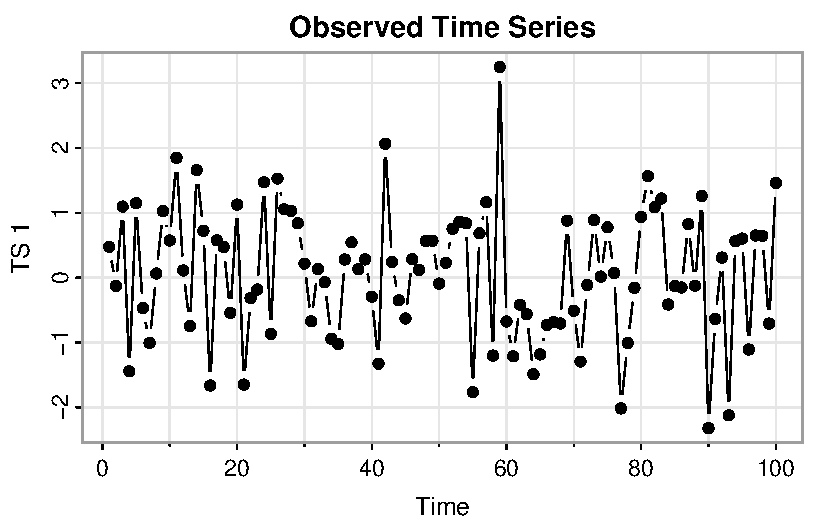
\includegraphics{Lecture7_files/figure-pdf/astsa_act2_part2-1.pdf}

\begin{Shaded}
\begin{Highlighting}[]
\FunctionTok{library}\NormalTok{(ggplot2)}
\FunctionTok{ggplot}\NormalTok{(all\_ts, }\FunctionTok{aes}\NormalTok{(}\AttributeTok{x =}\NormalTok{ Time, }\AttributeTok{y =}\NormalTok{ x\_t)) }\SpecialCharTok{+} \FunctionTok{geom\_point}\NormalTok{() }\SpecialCharTok{+} \FunctionTok{geom\_line}\NormalTok{() }\SpecialCharTok{+} \FunctionTok{ylab}\NormalTok{(}\StringTok{"TS 1"}\NormalTok{) }\SpecialCharTok{+} \FunctionTok{ggtitle}\NormalTok{(}\StringTok{"Observed Time Series \#1"}\NormalTok{)}
\end{Highlighting}
\end{Shaded}

\begin{enumerate}
\def\labelenumi{\arabic{enumi}.}
\setcounter{enumi}{2}
\tightlist
\item
  In separate plot, again plot the time series as just points and also
  plot a moving average smoother over the time series (use any \(p\)
  you'd like, but use a symmetric one). Create a data frame called
  \texttt{all\_ts} with the original time series and the moving average
  smoother.
\end{enumerate}

\begin{Shaded}
\begin{Highlighting}[]
\FunctionTok{tsplot}\NormalTok{(all\_ts}\SpecialCharTok{$}\NormalTok{x\_t, }\AttributeTok{type =} \StringTok{"b"}\NormalTok{, }\AttributeTok{ylab =} \StringTok{"TS 1"}\NormalTok{, }\AttributeTok{main =} \StringTok{"Moving Average Smoother (5 point)"}\NormalTok{, }\AttributeTok{pch =} \DecValTok{16}\NormalTok{ )}
\NormalTok{all\_ts}\SpecialCharTok{$}\NormalTok{ma\_x\_t }\OtherTok{\textless{}{-}}\NormalTok{ stats}\SpecialCharTok{::}\FunctionTok{filter}\NormalTok{(x\_t, }\AttributeTok{filter =}\FunctionTok{rep}\NormalTok{(}\DecValTok{1}\SpecialCharTok{/}\DecValTok{5}\NormalTok{,}\DecValTok{5}\NormalTok{), }\AttributeTok{sides =} \DecValTok{2}\NormalTok{)}
\FunctionTok{lines}\NormalTok{(all\_ts}\SpecialCharTok{$}\NormalTok{ma\_x\_t, }\AttributeTok{col =} \StringTok{"magenta"}\NormalTok{, }\AttributeTok{lwd =} \DecValTok{2}\NormalTok{)}
\end{Highlighting}
\end{Shaded}

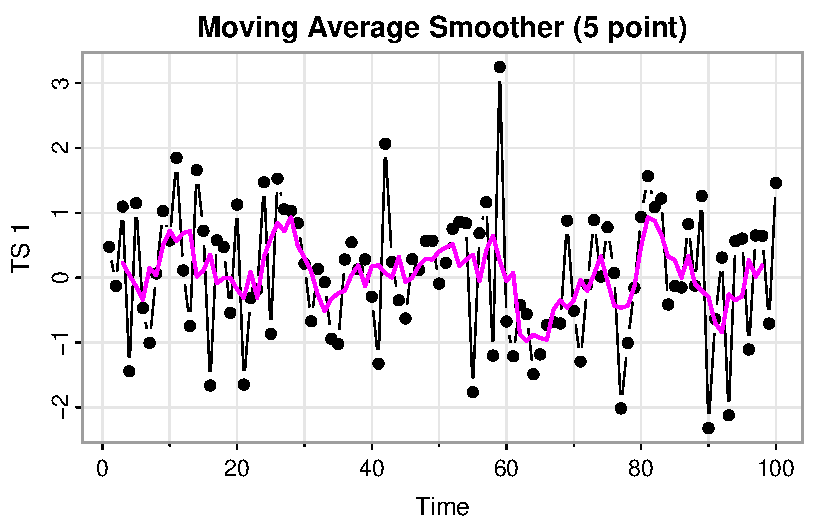
\includegraphics{Lecture7_files/figure-pdf/astsa_act2_p3-1.pdf}

\begin{Shaded}
\begin{Highlighting}[]
\FunctionTok{ggplot}\NormalTok{(all\_ts, }\FunctionTok{aes}\NormalTok{(}\AttributeTok{x =}\NormalTok{ Time, }\AttributeTok{y =}\NormalTok{ x\_t)) }\SpecialCharTok{+} \FunctionTok{geom\_point}\NormalTok{() }\SpecialCharTok{+} \FunctionTok{geom\_line}\NormalTok{() }\SpecialCharTok{+} 
  \FunctionTok{geom\_line}\NormalTok{(}\FunctionTok{aes}\NormalTok{(}\AttributeTok{x=}\NormalTok{ Time, }\AttributeTok{y =}\NormalTok{ ma\_x\_t), }\AttributeTok{col =} \StringTok{"magenta"}\NormalTok{) }\SpecialCharTok{+}
  \FunctionTok{ylab}\NormalTok{(}\StringTok{"TS 1"}\NormalTok{) }\SpecialCharTok{+} \FunctionTok{ggtitle}\NormalTok{(}\StringTok{"Detrended {-} Moving Average Smoother (5 point)"}\NormalTok{)}
\end{Highlighting}
\end{Shaded}

\begin{enumerate}
\def\labelenumi{\arabic{enumi}.}
\setcounter{enumi}{3}
\tightlist
\item
  \emph{Detrend} the time series with respect to the moving average
  estimate and plot the de-trended time series as points and lines. Save
  the detrended series in \texttt{all\_ts}.
\end{enumerate}

\begin{Shaded}
\begin{Highlighting}[]
\NormalTok{all\_ts}\SpecialCharTok{$}\NormalTok{detrended\_ma }\OtherTok{\textless{}{-}}\NormalTok{ all\_ts}\SpecialCharTok{$}\NormalTok{x\_t }\SpecialCharTok{{-}}\NormalTok{ all\_ts}\SpecialCharTok{$}\NormalTok{ma\_x\_t}

\FunctionTok{tsplot}\NormalTok{(all\_ts}\SpecialCharTok{$}\NormalTok{detrended, }\AttributeTok{type =} \StringTok{"b"}\NormalTok{, }\AttributeTok{ylab =} \StringTok{"TS 1"}\NormalTok{, }\AttributeTok{main =} \StringTok{"Detrended {-} Moving Average Smoother (5 point)"}\NormalTok{, }\AttributeTok{pch =} \DecValTok{16}\NormalTok{ )}
\end{Highlighting}
\end{Shaded}

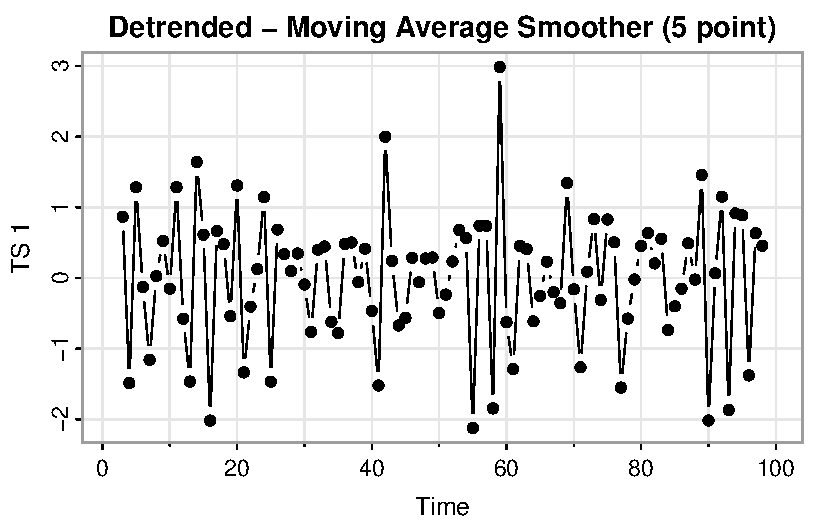
\includegraphics{Lecture7_files/figure-pdf/astsa_act2_p4-1.pdf}

\begin{Shaded}
\begin{Highlighting}[]
\FunctionTok{ggplot}\NormalTok{(all\_ts, }\FunctionTok{aes}\NormalTok{(}\AttributeTok{x =}\NormalTok{ Time, }\AttributeTok{y =}\NormalTok{ detrended\_ma)) }\SpecialCharTok{+} \FunctionTok{geom\_point}\NormalTok{() }\SpecialCharTok{+} \FunctionTok{geom\_line}\NormalTok{() }\SpecialCharTok{+} 
  \FunctionTok{ylab}\NormalTok{(}\StringTok{"TS 1"}\NormalTok{) }\SpecialCharTok{+} \FunctionTok{ggtitle}\NormalTok{(}\StringTok{"Detrended {-} Moving Average Smoother (5 point)"}\NormalTok{)}
\end{Highlighting}
\end{Shaded}

\begin{enumerate}
\def\labelenumi{\arabic{enumi}.}
\setcounter{enumi}{4}
\tightlist
\item
  In a separate plot, again plot the time series as points and also plot
  a simple linear regression line using \texttt{time(x)} where x is the
  time series you are analyzing. Add the fitted values to the
  \texttt{all\_ts} data frame.
\end{enumerate}

\begin{Shaded}
\begin{Highlighting}[]
\NormalTok{lm\_x\_t }\OtherTok{\textless{}{-}} \FunctionTok{lm}\NormalTok{(x\_t}\SpecialCharTok{\textasciitilde{}}\NormalTok{Time, }\AttributeTok{data =}\NormalTok{ all\_ts)}
\FunctionTok{tsplot}\NormalTok{(all\_ts}\SpecialCharTok{$}\NormalTok{x\_t, }\AttributeTok{type =} \StringTok{"b"}\NormalTok{, }\AttributeTok{ylab =} \StringTok{"TS 1"}\NormalTok{, }\AttributeTok{main =} \StringTok{"Linear Trend"}\NormalTok{, }\AttributeTok{pch =} \DecValTok{16}\NormalTok{)}
\NormalTok{all\_ts}\SpecialCharTok{$}\NormalTok{reg\_x\_t }\OtherTok{\textless{}{-}}\NormalTok{ lm\_x\_t}\SpecialCharTok{$}\NormalTok{fitted.values}
\FunctionTok{lines}\NormalTok{(all\_ts}\SpecialCharTok{$}\NormalTok{reg\_x\_t, }\AttributeTok{col =} \StringTok{"turquoise"}\NormalTok{, }\AttributeTok{lwd =} \DecValTok{2}\NormalTok{)}
\end{Highlighting}
\end{Shaded}

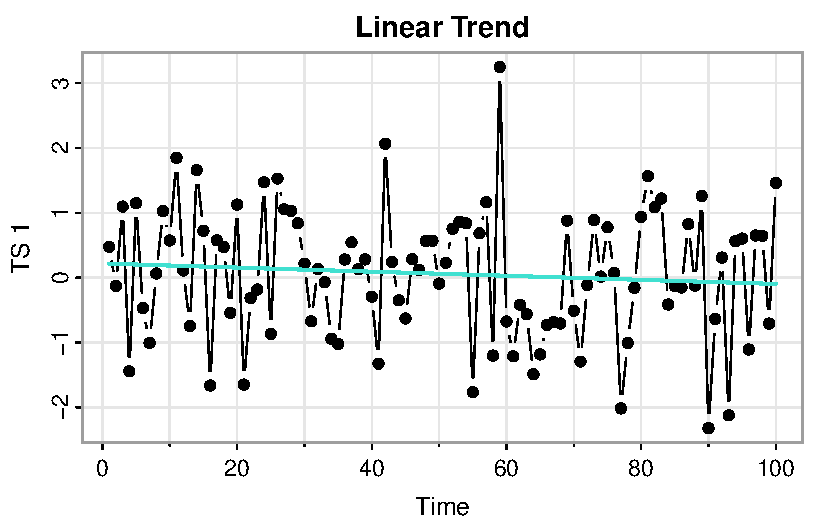
\includegraphics{Lecture7_files/figure-pdf/astsa_act2_part5-1.pdf}

\begin{Shaded}
\begin{Highlighting}[]
\FunctionTok{ggplot}\NormalTok{(all\_ts, }\FunctionTok{aes}\NormalTok{(}\AttributeTok{x =}\NormalTok{ Time, }\AttributeTok{y =}\NormalTok{ x\_t)) }\SpecialCharTok{+} \FunctionTok{geom\_point}\NormalTok{() }\SpecialCharTok{+} \FunctionTok{geom\_line}\NormalTok{() }\SpecialCharTok{+} 
  \FunctionTok{ylab}\NormalTok{(}\StringTok{"TS 1"}\NormalTok{) }\SpecialCharTok{+} \FunctionTok{ggtitle}\NormalTok{(}\StringTok{"Linear Trend"}\NormalTok{) }\SpecialCharTok{+} \FunctionTok{geom\_line}\NormalTok{(}\FunctionTok{aes}\NormalTok{(}\AttributeTok{x=}\NormalTok{ Time, }\AttributeTok{y =}\NormalTok{ reg\_x\_t), }\AttributeTok{col =} \StringTok{"turquoise"}\NormalTok{) }
\end{Highlighting}
\end{Shaded}

\begin{enumerate}
\def\labelenumi{\arabic{enumi}.}
\setcounter{enumi}{5}
\tightlist
\item
  Detrend the time series with respect to the regression and plot and
  save the detrended series (save in the all\_ts data frame).
\end{enumerate}

\begin{Shaded}
\begin{Highlighting}[]
\NormalTok{all\_ts}\SpecialCharTok{$}\NormalTok{detrended\_reg }\OtherTok{\textless{}{-}}\NormalTok{ all\_ts}\SpecialCharTok{$}\NormalTok{x\_t }\SpecialCharTok{{-}}\NormalTok{ all\_ts}\SpecialCharTok{$}\NormalTok{reg\_x\_t}
\FunctionTok{tsplot}\NormalTok{(all\_ts}\SpecialCharTok{$}\NormalTok{detrended\_reg, }\AttributeTok{type =} \StringTok{"b"}\NormalTok{, }\AttributeTok{ylab =} \StringTok{"TS 1"}\NormalTok{, }\AttributeTok{main =} \StringTok{"Detrended {-} Linear Trend"}\NormalTok{, }\AttributeTok{pch =} \DecValTok{16}\NormalTok{ )}
\end{Highlighting}
\end{Shaded}

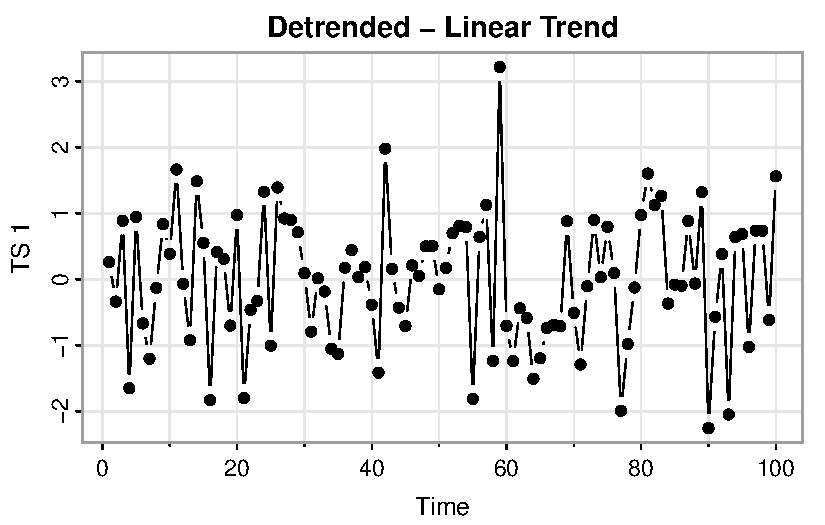
\includegraphics{Lecture7_files/figure-pdf/astsa-act2-p6-1.pdf}

\begin{Shaded}
\begin{Highlighting}[]
\FunctionTok{ggplot}\NormalTok{(all\_ts, }\FunctionTok{aes}\NormalTok{(}\AttributeTok{x =}\NormalTok{ Time, }\AttributeTok{y =}\NormalTok{ detrended\_reg)) }\SpecialCharTok{+} \FunctionTok{geom\_point}\NormalTok{() }\SpecialCharTok{+} \FunctionTok{geom\_line}\NormalTok{() }\SpecialCharTok{+} 
  \FunctionTok{ylab}\NormalTok{(}\StringTok{"TS 1"}\NormalTok{) }\SpecialCharTok{+} \FunctionTok{ggtitle}\NormalTok{(}\StringTok{"Detrended {-} Linear Trend"}\NormalTok{)}
\end{Highlighting}
\end{Shaded}

\begin{enumerate}
\def\labelenumi{\arabic{enumi}.}
\setcounter{enumi}{6}
\tightlist
\item
  Difference the time series, plot as points and lines and save the
  differenced series.
\end{enumerate}

\begin{Shaded}
\begin{Highlighting}[]
\NormalTok{all\_ts}\SpecialCharTok{$}\NormalTok{differenced }\OtherTok{\textless{}{-}} \FunctionTok{c}\NormalTok{(}\FunctionTok{diff}\NormalTok{(all\_ts}\SpecialCharTok{$}\NormalTok{x\_t), }\ConstantTok{NA}\NormalTok{)}
\FunctionTok{tsplot}\NormalTok{(all\_ts}\SpecialCharTok{$}\NormalTok{differenced, }\AttributeTok{type =} \StringTok{"b"}\NormalTok{, }\AttributeTok{ylab =} \StringTok{"TS 1"}\NormalTok{, }\AttributeTok{main =} \StringTok{"Differenced Series"}\NormalTok{, }\AttributeTok{pch =} \DecValTok{16}\NormalTok{ )}
\end{Highlighting}
\end{Shaded}

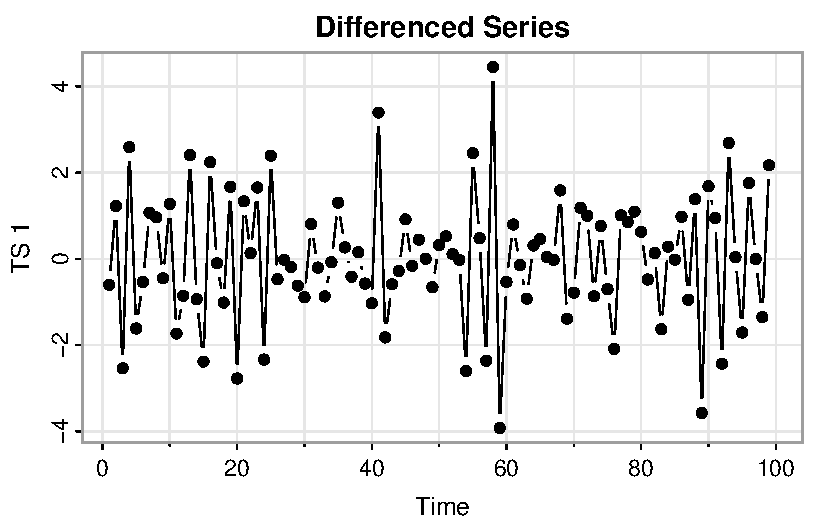
\includegraphics{Lecture7_files/figure-pdf/astsa-act2-p7-1.pdf}

\begin{Shaded}
\begin{Highlighting}[]
\FunctionTok{ggplot}\NormalTok{(all\_ts, }\FunctionTok{aes}\NormalTok{(}\AttributeTok{x =}\NormalTok{ Time, }\AttributeTok{y =}\NormalTok{ differenced)) }\SpecialCharTok{+} \FunctionTok{geom\_point}\NormalTok{() }\SpecialCharTok{+} 
  \FunctionTok{ylab}\NormalTok{(}\StringTok{"TS 1"}\NormalTok{) }\SpecialCharTok{+} \FunctionTok{ggtitle}\NormalTok{(}\StringTok{"Differenced Series"}\NormalTok{)}
\end{Highlighting}
\end{Shaded}

\begin{enumerate}
\def\labelenumi{\arabic{enumi}.}
\setcounter{enumi}{6}
\tightlist
\item
  \texttt{Run\ par(mfrow\ =\ c(2,3))} and then re-run the plotting code
  for all 6 plots you just made in steps 1-6.
\end{enumerate}

\begin{Shaded}
\begin{Highlighting}[]
\FunctionTok{par}\NormalTok{(}\AttributeTok{mfrow =} \FunctionTok{c}\NormalTok{(}\DecValTok{2}\NormalTok{,}\DecValTok{3}\NormalTok{))}
 
\CommentTok{\# number 1}
\FunctionTok{tsplot}\NormalTok{(all\_ts}\SpecialCharTok{$}\NormalTok{x\_t, }\AttributeTok{type =} \StringTok{"b"}\NormalTok{, }\AttributeTok{ylab =} \StringTok{"TS 1"}\NormalTok{, }\AttributeTok{main =} \StringTok{"Observed Time Series"}\NormalTok{, }\AttributeTok{pch =} \DecValTok{16}\NormalTok{)}
  
\DocumentationTok{\#\# number 2}
\FunctionTok{tsplot}\NormalTok{(all\_ts}\SpecialCharTok{$}\NormalTok{x\_t, }\AttributeTok{type =} \StringTok{"b"}\NormalTok{, }\AttributeTok{ylab =} \StringTok{"TS 1"}\NormalTok{, }\AttributeTok{main =} \StringTok{"MA(5) Smoother"}\NormalTok{, }\AttributeTok{pch =} \DecValTok{16}\NormalTok{ )}
\FunctionTok{lines}\NormalTok{(all\_ts}\SpecialCharTok{$}\NormalTok{ma\_x\_t, }\AttributeTok{col =} \StringTok{"magenta"}\NormalTok{, }\AttributeTok{lwd =} \DecValTok{2}\NormalTok{)}
\CommentTok{\# number 3}
\FunctionTok{tsplot}\NormalTok{(all\_ts}\SpecialCharTok{$}\NormalTok{detrended\_ma, }\AttributeTok{type =} \StringTok{"b"}\NormalTok{, }\AttributeTok{ylab =} \StringTok{"TS 1"}\NormalTok{, }\AttributeTok{main =} \StringTok{"Detrended {-} MA(5)"}\NormalTok{, }\AttributeTok{pch =} \DecValTok{16}\NormalTok{ )}
\CommentTok{\# Number 4}
\FunctionTok{tsplot}\NormalTok{(all\_ts}\SpecialCharTok{$}\NormalTok{x\_t, }\AttributeTok{type =} \StringTok{"b"}\NormalTok{, }\AttributeTok{ylab =} \StringTok{"TS 1"}\NormalTok{, }\AttributeTok{main =} \StringTok{"Linear Trend"}\NormalTok{, }\AttributeTok{pch =} \DecValTok{16}\NormalTok{)}
\FunctionTok{lines}\NormalTok{(all\_ts}\SpecialCharTok{$}\NormalTok{reg\_x\_t, }\AttributeTok{col =} \StringTok{"turquoise"}\NormalTok{, }\AttributeTok{lwd =} \DecValTok{2}\NormalTok{)}
  
\CommentTok{\# number 5}
\FunctionTok{tsplot}\NormalTok{(all\_ts}\SpecialCharTok{$}\NormalTok{detrended\_reg, }\AttributeTok{type =} \StringTok{"b"}\NormalTok{, }\AttributeTok{ylab =} \StringTok{"TS 1"}\NormalTok{, }\AttributeTok{main =} \StringTok{"Detrended {-} Linear Trend"}\NormalTok{, }\AttributeTok{pch =} \DecValTok{16}\NormalTok{)}

\CommentTok{\# Number 6}
\FunctionTok{tsplot}\NormalTok{(all\_ts}\SpecialCharTok{$}\NormalTok{differenced, }\AttributeTok{type =} \StringTok{"b"}\NormalTok{, }\AttributeTok{ylab =} \StringTok{"TS 1"}\NormalTok{, }\AttributeTok{main =} \StringTok{"Differenced"}\NormalTok{, }\AttributeTok{pch =} \DecValTok{16}\NormalTok{ )}
\end{Highlighting}
\end{Shaded}

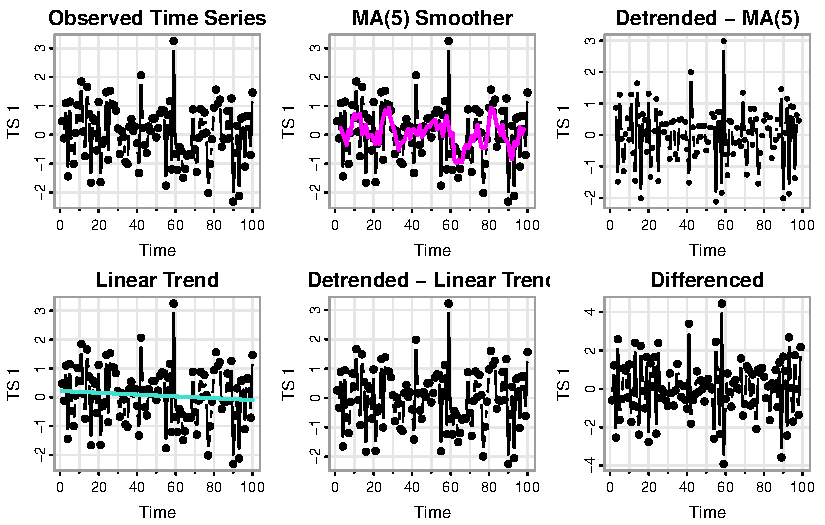
\includegraphics{Lecture7_files/figure-pdf/all_parts-1.pdf}

\subsubsection{Short answer answers}\label{short-answer-answers}

\begin{itemize}
\tightlist
\item
  Which plots look like stationary time series?
\end{itemize}

\textbf{In terms of the ``data'' (black points/lines in upper left and
middle and lower left), the plot looks fairly stationary-- no increasing
or cyclical trend, and looks fairly similar to white noise (which is
stationary). The detrended (MA and Linear) and the differenced plots
look very similar, so they seem stationary as well.}

\textbf{In terms of the time series generated from creating trend
estimates from each time point, we have two: the MA(5) and the linear
trend. The linear trend is very slightly negative, but essentially
horizontal-- stationary.}

\textbf{The MA(5) smoother has fluctuations but those don't seem to be
explicitly based directly on time (or for particular time lags, i.e.~not
seasonal), which would suggest stationarity (though perhaps some
temporal structure-- we can check the acf.)}

\begin{tcolorbox}[enhanced jigsaw, left=2mm, opacitybacktitle=0.6, coltitle=black, title=\textcolor{quarto-callout-note-color}{\faInfo}\hspace{0.5em}{Regression significance tests that suggest white noise.}, rightrule=.15mm, colbacktitle=quarto-callout-note-color!10!white, opacityback=0, toptitle=1mm, toprule=.15mm, breakable, bottomtitle=1mm, titlerule=0mm, colback=white, arc=.35mm, bottomrule=.15mm, leftrule=.75mm, colframe=quarto-callout-note-color-frame]

Running \texttt{summary(lm\_x\_t)} contains the test statistics and
p-values for some hypothesis tests for the regression parameters.

\begin{itemize}
\tightlist
\item
  Here, we have a p-value of 0.369 for the test for a zero slope,
  meaning we do not have evidence the slope of the trend is not zero.
\item
  The default test of significance for the y-intercept is actually
  testing whether it's 0, and that we also fail to reject that the
  y-intercept is different from 0 (p-value 0.285.
\end{itemize}

In other words, we fail to find evidence that the mean is not constant
and 0, which is true for white noise. So it kinda seems like white
noise.

\end{tcolorbox}

\begin{itemize}
\tightlist
\item
  Can you guess the model/source of \(x_t\) from these plots?
\end{itemize}

\textbf{It looks like white noise, but the acf can give us more insight
into that in Activity 4.}

\begin{itemize}
\tightlist
\item
  How many trends have we estimated?
\end{itemize}

\textbf{We have estimated two trends. Note that differencing a series
does not give us an estimate of the trend.}

\subsection{Activity 3}\label{activity-3}

Use the function \texttt{process\_ts} to create the plots for the
remaining series.

\textbf{Note that we estimate the same two trend models (MA(5) and
linear) for each series (though the particular parameters will be
different for each of the raw series).}

\begin{Shaded}
\begin{Highlighting}[]
\FunctionTok{source}\NormalTok{(}\StringTok{"Code/process\_ts.r"}\NormalTok{)}
\end{Highlighting}
\end{Shaded}

\begin{Shaded}
\begin{Highlighting}[]
\FunctionTok{process\_ts}\NormalTok{(time\_series}\SpecialCharTok{$}\NormalTok{y1, }\AttributeTok{ptitle =} \StringTok{"TS1"}\NormalTok{)}
\end{Highlighting}
\end{Shaded}

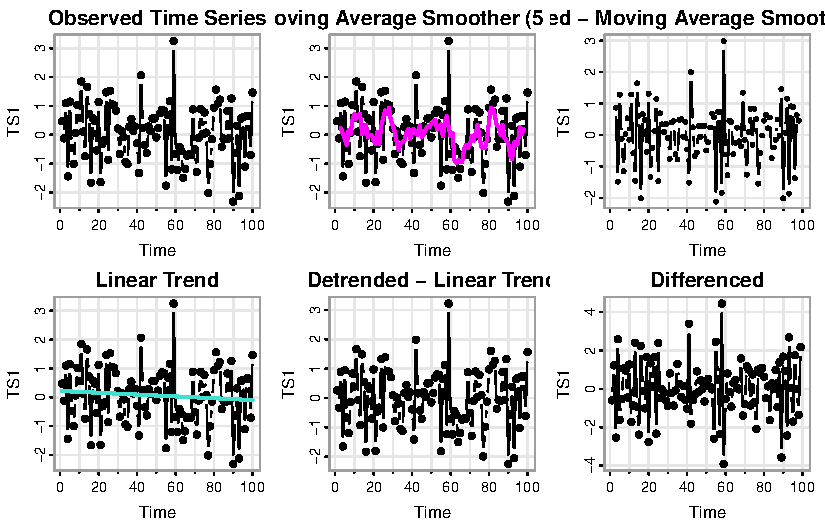
\includegraphics{Lecture7_files/figure-pdf/unnamed-chunk-16-1.pdf}

\begin{itemize}
\tightlist
\item
  Which plots look like stationary time series?
\end{itemize}

\textbf{see above}

\begin{itemize}
\tightlist
\item
  Can you guess the model/source of \(x_t\) from these plots?
\end{itemize}

\textbf{see above}

\begin{Shaded}
\begin{Highlighting}[]
\FunctionTok{process\_ts}\NormalTok{(time\_series}\SpecialCharTok{$}\NormalTok{y2, }\AttributeTok{ptitle =} \StringTok{"TS2"}\NormalTok{)}
\end{Highlighting}
\end{Shaded}

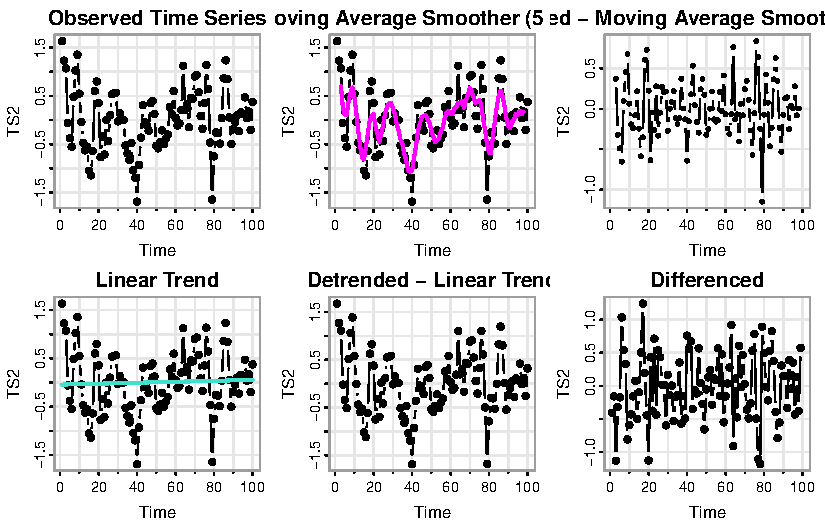
\includegraphics{Lecture7_files/figure-pdf/unnamed-chunk-17-1.pdf}

\begin{itemize}
\item
  Which plots look like stationary time series?
\item
  The detrended MA and differenced series look very much like white
  noise, which implies stationary.
\item
  The detrended linear trend is almost identical to the raw data (which
  makes sense since the linear regression estimates essentially a
  constant mean of 0).
\item
  The raw data does not appear to have an overall increasing trend, nor
  any predictable seasonal patterns (not a linear trend stationary,
  unless I was being mean). However, it does not really look like white
  noise.
\end{itemize}

So that means \texttt{y2} may be a moving average or perhaps real data.

\begin{tcolorbox}[enhanced jigsaw, left=2mm, opacitybacktitle=0.6, coltitle=black, title=\textcolor{quarto-callout-note-color}{\faInfo}\hspace{0.5em}{How I could have been mean}, rightrule=.15mm, colbacktitle=quarto-callout-note-color!10!white, opacityback=0, toptitle=1mm, toprule=.15mm, breakable, bottomtitle=1mm, titlerule=0mm, colback=white, arc=.35mm, bottomrule=.15mm, leftrule=.75mm, colframe=quarto-callout-note-color-frame]

Technically, a (deterministic) linear trend stationary model with the
usual regression residuals with mean and y-intercept 0 is equivalent to
white noise.

\end{tcolorbox}

\begin{itemize}
\tightlist
\item
  Can you guess the model/source of \(x_t\) from these plots?
\end{itemize}

Not exactly! The Acf will reveal more about the temporal structure.

\begin{Shaded}
\begin{Highlighting}[]
\FunctionTok{process\_ts}\NormalTok{(time\_series}\SpecialCharTok{$}\NormalTok{y3, }\AttributeTok{ptitle =} \StringTok{"TS3"}\NormalTok{)}
\end{Highlighting}
\end{Shaded}

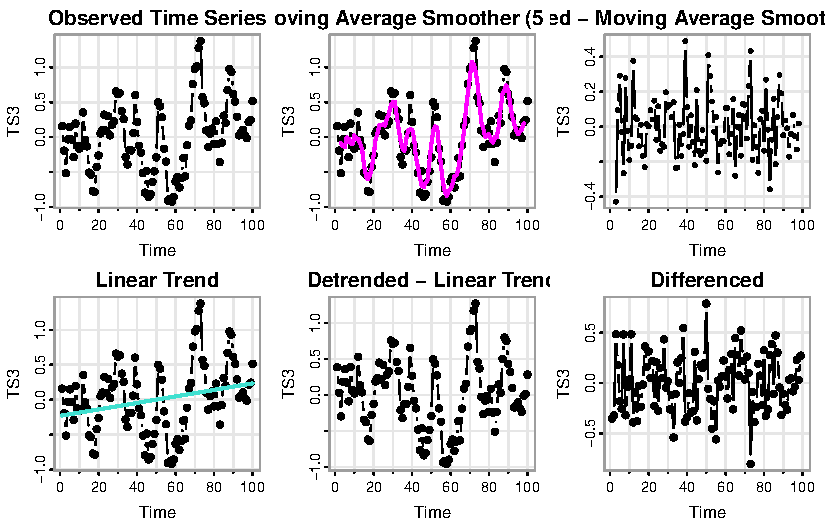
\includegraphics{Lecture7_files/figure-pdf/unnamed-chunk-18-1.pdf}

\begin{itemize}
\tightlist
\item
  Which plots look like stationary time series?
\item
  Can you guess the model/source of \(x_t\) from these plots?
\end{itemize}

\textbf{(Answering both) The plots for \texttt{y3} are somewhat similar
to those for \texttt{y2}, so this may be the duplicated model (not white
noise, though). However, there are some differences. The linear trend is
more pronounced, but still appears somewhat shallow. Looking at the raw
series, the appearance of temporal structure is even more pronounced.
So, perhaps this the deterministic linear model with a very shallow
trend (technically still nonstationary), or it's a moving average, or
real data.}

\begin{Shaded}
\begin{Highlighting}[]
\FunctionTok{process\_ts}\NormalTok{(time\_series}\SpecialCharTok{$}\NormalTok{y4, }\AttributeTok{ptitle =} \StringTok{"TS4"}\NormalTok{)}
\end{Highlighting}
\end{Shaded}

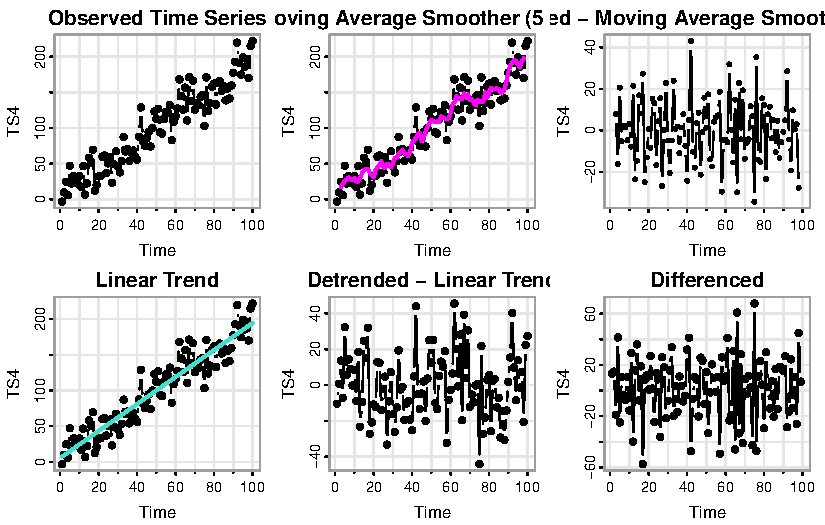
\includegraphics{Lecture7_files/figure-pdf/unnamed-chunk-19-1.pdf}

\begin{itemize}
\tightlist
\item
  Which plots look like stationary time series?
\end{itemize}

The detrended and differenced plots look stationary. The observed time
series looks like an obvious deterministic linear trend, which the
linear trend and moving average trend pick up on (though the moving
average is a ``bumpy'' estimate of the linear trend-- but there does not
appear to be any cyclical structure.)

\begin{itemize}
\tightlist
\item
  Can you guess the model/source of \(x_t\) from these plots?
\end{itemize}

\textbf{This could technically be real data, if that real data followed
a perfect linear trend in time. It's definitely not white noise or a
pure moving average model (generated from white noise).}

\begin{Shaded}
\begin{Highlighting}[]
\FunctionTok{process\_ts}\NormalTok{(time\_series}\SpecialCharTok{$}\NormalTok{y5, }\AttributeTok{ptitle =} \StringTok{"TS5"}\NormalTok{)}
\end{Highlighting}
\end{Shaded}

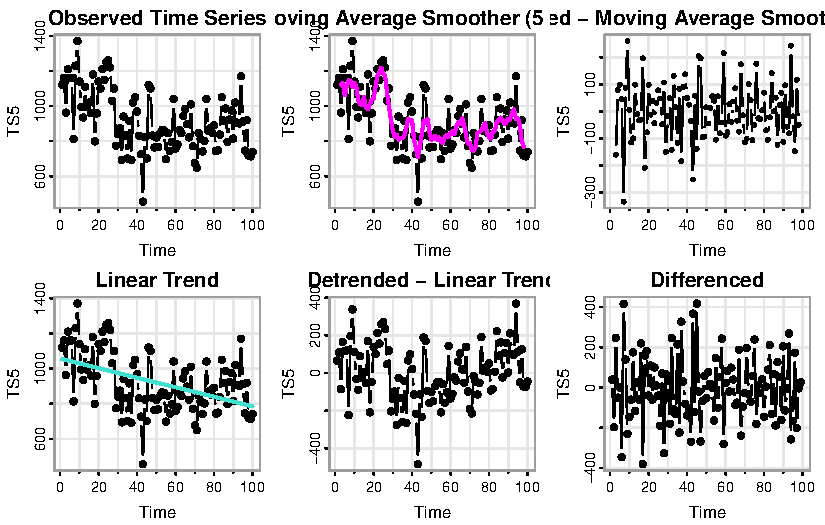
\includegraphics{Lecture7_files/figure-pdf/unnamed-chunk-20-1.pdf}

\begin{itemize}
\tightlist
\item
  Which plots look like stationary time series?
\end{itemize}

\textbf{The MA-detrended and differenced series look stationary. The raw
data looks like it is at one level for the beginning of the series and
then drops down for the remainder. That pattern is more pronounced in
the moving average overaly plot. The linear trend is decreasing, but
does not appear to capture the pattern of the data very well (the
decrease in the data is abrupt, not linear and gradual).}

\begin{itemize}
\tightlist
\item
  Can you guess the model/source of \(x_t\) from these plots?
\end{itemize}

\textbf{None of the models (moving average, linear trend, white noise)
can have an abrupt change in level like we see in this time series. By
process of elimination, this appears to be the real data.}

\subsection{Activity 4}\label{activity-4}

\begin{Shaded}
\begin{Highlighting}[]
\FunctionTok{library}\NormalTok{(patchwork)}
\NormalTok{plot\_acfs }\OtherTok{\textless{}{-}} \ControlFlowTok{function}\NormalTok{(dataset, main)\{}
  
\NormalTok{  all\_ts }\OtherTok{\textless{}{-}} \FunctionTok{process\_ts}\NormalTok{(dataset, }\AttributeTok{ptitle =} \StringTok{""}\NormalTok{, }\AttributeTok{output =}\NormalTok{ T, }\AttributeTok{plots =}\NormalTok{ F)}
  
\NormalTok{  p }\OtherTok{\textless{}{-}}\NormalTok{  forecast}\SpecialCharTok{::}\FunctionTok{ggAcf}\NormalTok{(all\_ts}\SpecialCharTok{$}\NormalTok{x\_t)  }\SpecialCharTok{+} \FunctionTok{ylim}\NormalTok{(}\SpecialCharTok{{-}}\DecValTok{1}\NormalTok{,}\DecValTok{1}\NormalTok{) }\SpecialCharTok{+} \FunctionTok{ggtitle}\NormalTok{(}\FunctionTok{names}\NormalTok{(all\_ts)[}\DecValTok{1}\NormalTok{]) }\SpecialCharTok{+}  \FunctionTok{plot\_layout}\NormalTok{(}\AttributeTok{nrow =} \DecValTok{2}\NormalTok{, }\AttributeTok{ncol =} \DecValTok{3}\NormalTok{)}
\ControlFlowTok{for}\NormalTok{(i }\ControlFlowTok{in} \FunctionTok{names}\NormalTok{(all\_ts)[}\SpecialCharTok{!}\NormalTok{(}\FunctionTok{names}\NormalTok{(all\_ts)}\SpecialCharTok{\%in\%} \FunctionTok{c}\NormalTok{(}\StringTok{"Time"}\NormalTok{, }\StringTok{"x\_t"}\NormalTok{))])\{}

\NormalTok{  g }\OtherTok{\textless{}{-}}\NormalTok{ forecast}\SpecialCharTok{::}\FunctionTok{ggAcf}\NormalTok{(all\_ts[, i])  }\SpecialCharTok{+} \FunctionTok{ylim}\NormalTok{(}\SpecialCharTok{{-}}\DecValTok{1}\NormalTok{,}\DecValTok{1}\NormalTok{) }\SpecialCharTok{+} \FunctionTok{ggtitle}\NormalTok{(i) }
\NormalTok{  p }\OtherTok{\textless{}{-}}\NormalTok{ p }\SpecialCharTok{+}\NormalTok{ g}\SpecialCharTok{+} \FunctionTok{plot\_layout}\NormalTok{(}\AttributeTok{nrow =} \DecValTok{2}\NormalTok{, }\AttributeTok{ncol =} \DecValTok{3}\NormalTok{) }\SpecialCharTok{+} \FunctionTok{plot\_annotation}\NormalTok{(}\AttributeTok{title =} \FunctionTok{paste}\NormalTok{(main))}
\NormalTok{\}}

\NormalTok{p}
\NormalTok{\}}
\end{Highlighting}
\end{Shaded}

\begin{Shaded}
\begin{Highlighting}[]
\FunctionTok{plot\_acfs}\NormalTok{(time\_series}\SpecialCharTok{$}\NormalTok{y1, }\AttributeTok{main =} \StringTok{"TS 1"}\NormalTok{)}
\end{Highlighting}
\end{Shaded}

\begin{verbatim}
Registered S3 method overwritten by 'quantmod':
  method            from
  as.zoo.data.frame zoo 
\end{verbatim}

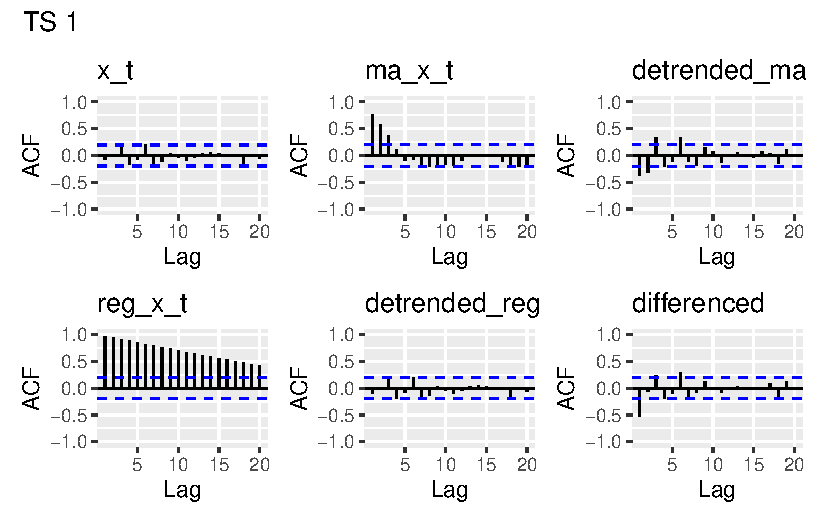
\includegraphics{Lecture7_files/figure-pdf/unnamed-chunk-22-1.pdf}

\begin{Shaded}
\begin{Highlighting}[]
\FunctionTok{plot\_acfs}\NormalTok{(time\_series}\SpecialCharTok{$}\NormalTok{y2, }\AttributeTok{main =} \StringTok{"TS 2"}\NormalTok{)}
\end{Highlighting}
\end{Shaded}

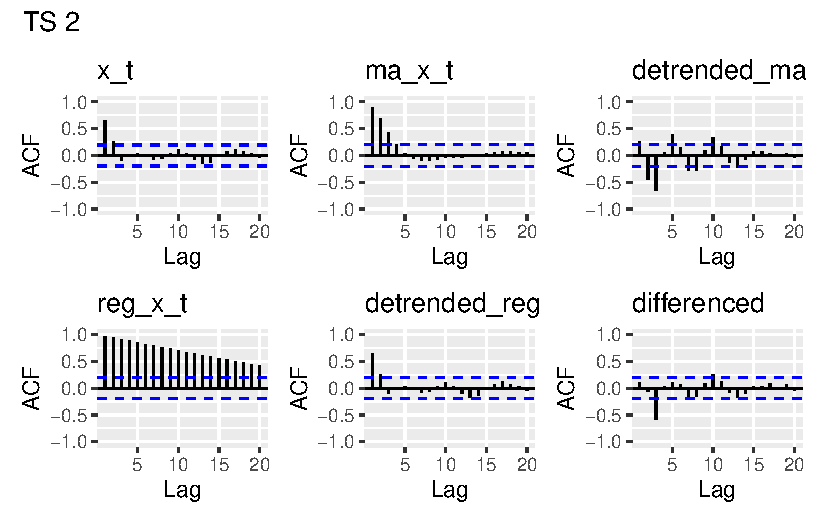
\includegraphics{Lecture7_files/figure-pdf/unnamed-chunk-22-2.pdf}

\begin{Shaded}
\begin{Highlighting}[]
\FunctionTok{plot\_acfs}\NormalTok{(time\_series}\SpecialCharTok{$}\NormalTok{y3, }\AttributeTok{main =} \StringTok{"TS 3"}\NormalTok{)}
\end{Highlighting}
\end{Shaded}

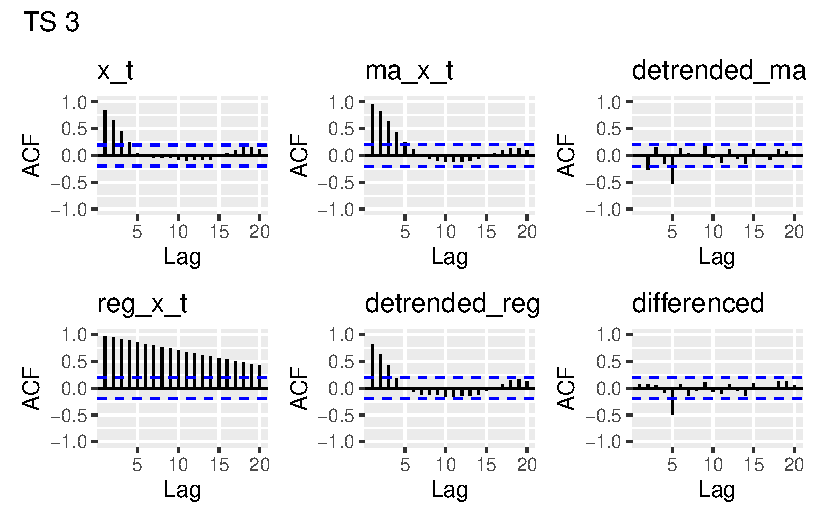
\includegraphics{Lecture7_files/figure-pdf/unnamed-chunk-22-3.pdf}

\begin{Shaded}
\begin{Highlighting}[]
\FunctionTok{plot\_acfs}\NormalTok{(time\_series}\SpecialCharTok{$}\NormalTok{y4, }\AttributeTok{main =} \StringTok{"TS 4"}\NormalTok{)}
\end{Highlighting}
\end{Shaded}

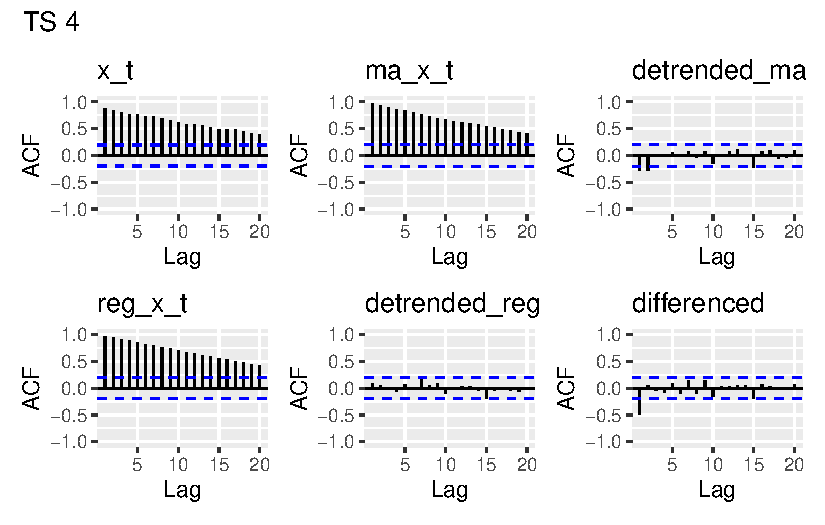
\includegraphics{Lecture7_files/figure-pdf/unnamed-chunk-22-4.pdf}

\begin{Shaded}
\begin{Highlighting}[]
\FunctionTok{plot\_acfs}\NormalTok{(time\_series}\SpecialCharTok{$}\NormalTok{y5, }\AttributeTok{main =} \StringTok{"TS 5"}\NormalTok{)}
\end{Highlighting}
\end{Shaded}

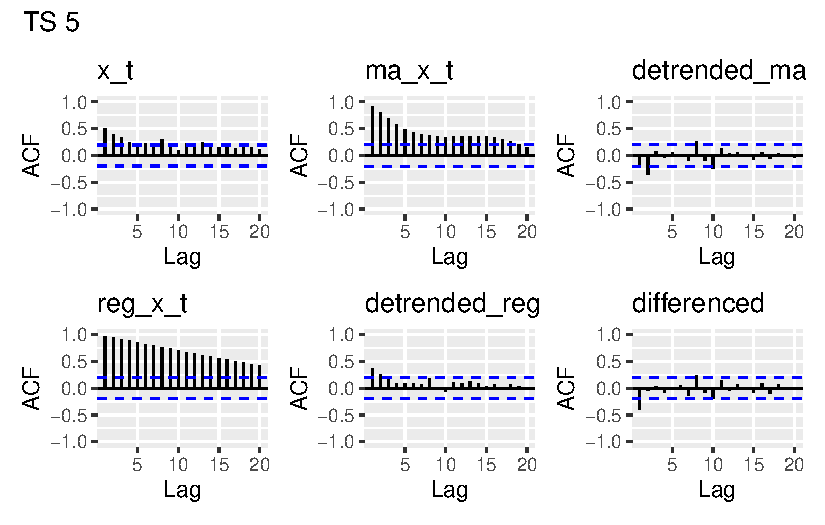
\includegraphics{Lecture7_files/figure-pdf/unnamed-chunk-22-5.pdf}

\paragraph{\texorpdfstring{ACF of the
\texttt{y}'s}{ACF of the y's}}\label{acf-of-the-ys}

\begin{itemize}
\tightlist
\item
  \texttt{y1}- looks like white noise
\item
  \texttt{y2}- clearly has lag 1 autocorrelation, maybe a but at lag 2,
  then drops off. A bit of a pattern in later lags
\item
  \texttt{y3}- has autocorrelation for lags 1-4, then drops off around
  5. A bit of a pattern in later lags like \texttt{y2}, but more
  pronounced than \texttt{y2}.
\item
  \texttt{y4}- This is the one we think is the linear trend model.
  Clearly there is nonstationarity in the acf of the data, which we'd
  expect to see from a linear trend.
\item
  \texttt{y5}- This looks unlike any of the others. There appears to be
  moderate lag 1 autocorrelation which drops off slowly.
\end{itemize}

\paragraph{ACF of the MA(5) estimates}\label{acf-of-the-ma5-estimates}

\begin{itemize}
\tightlist
\item
  \texttt{y1}- Since it appears we started with white noise, it makes
  sense that we can clearly identify a moving average structure in the
  time series that we made by applying a moving average. We are seeing
  the structure we built into our MA(5) trend estimate.
\item
  \texttt{y2}- Looks very similar to \texttt{y1}.
\item
  \texttt{y3}- Similar to the first two, but has larger autocorrelation
  for lags 1-4.
\item
  \texttt{y4}- Looks the same as the acf of \texttt{y4}, and drops off
  very slowly. Our MA estimate essentially is a linear trend, so it's
  not surprising to see this structure in the acf.
\item
  \texttt{y5}- Again, this looks like none of the others. We see the
  larger autocorrelation at small lags induced by the MA smoothing, but
  we also see more persistent long-range lag relations.
\end{itemize}

\paragraph{ACF of the MA-5 detrended}\label{acf-of-the-ma-5-detrended}

None of the MA(5)- detrended series look particularly like white noise,
which is what we would want to see if we had fully accounted for the
temporal structure in our model.

\begin{itemize}
\tightlist
\item
  \texttt{y1}- has some temporal structure, likely due to the fact that
  we appear to have started with white noise and then subtracted out the
  MA structure
\item
  \texttt{y2}- has even more structure than \texttt{y1}
\item
  \texttt{y3}- looks like white noise, except for a peak at \texttt{y5}
\item
  \texttt{y4}- looks almost like white noise, except for lag 1 and 2
  showing some modest negative autocorrelation
\item
  \texttt{y5}- looks kind of like the white noise, but perhaps has a bit
  of structure
\end{itemize}

\paragraph{ACF of the linear trends}\label{acf-of-the-linear-trends}

These all look very similar. That is because each of our linear trend
models are deterministic functions of \(t\)-- they will show this
autocorrelation regardless of the steepness of the slope (unless it's
literally 0).

\paragraph{ACF of the linearly
detrended}\label{acf-of-the-linearly-detrended}

\begin{itemize}
\tightlist
\item
  \texttt{y1}- Looks like white noise-- unsurprising since we subtracted
  off a near horizontal trend of 0, and we suspect a linear model
\item
  \texttt{y2}- has significant autocorrelation at lag 1-- looks like the
  regression does \emph{not} have independent errors, so probably not a
  great model
\item
  \texttt{y3}- same as \texttt{y2}, but has a larger autocorrelation and
  for lags 2 and 3 as well
\item
  \texttt{y4}- Looks like white noise-- unsurprising since we linearly
  detrended and we suspect a linear model.
\item
  \texttt{y5}- Not quite like white noise (most autocorrelations are
  small but positive), but doesn't look too bad.
\end{itemize}

\paragraph{ACF of the differences}\label{acf-of-the-differences}

\begin{itemize}
\tightlist
\item
  \texttt{y1}- Significant lag 1 autocorrelation (makes sense since we
  differenced white noise, which added some dependence)
\item
  \texttt{y2}- Significant lag 3 autocorrelation
\item
  \texttt{y3}- Significant lag 5 autocorrelation
\item
  \texttt{y4}- some lag 1 autocorrelation
\item
  \texttt{y5}- some lag 1 autocorrelation
\end{itemize}

\subsection{Simulation solutions.}\label{simulation-solutions.}

\begin{Shaded}
\begin{Highlighting}[]
\FunctionTok{set.seed}\NormalTok{(}\DecValTok{0016}\NormalTok{)}
\NormalTok{N }\OtherTok{\textless{}{-}} \DecValTok{100}
\DocumentationTok{\#\# Simulate white noise.}
\NormalTok{y1 }\OtherTok{\textless{}{-}} \FunctionTok{rnorm}\NormalTok{(N)}

\DocumentationTok{\#\# Simulate an MA(3) }
\NormalTok{w }\OtherTok{\textless{}{-}} \FunctionTok{rnorm}\NormalTok{(N}\SpecialCharTok{+}\DecValTok{50}\NormalTok{)}
\NormalTok{y2 }\OtherTok{\textless{}{-}}\NormalTok{ stats}\SpecialCharTok{::}\FunctionTok{filter}\NormalTok{(w, }\AttributeTok{filter =} \FunctionTok{rep}\NormalTok{(}\DecValTok{1}\SpecialCharTok{/}\DecValTok{3}\NormalTok{,}\DecValTok{3}\NormalTok{), }
                    \AttributeTok{method =} \StringTok{"convolution"}\NormalTok{, }\AttributeTok{sides =} \DecValTok{2}\NormalTok{)[}\DecValTok{2}\SpecialCharTok{:}\DecValTok{101}\NormalTok{]}
\DocumentationTok{\#\# Simulate an MA(5)}
\NormalTok{w }\OtherTok{\textless{}{-}} \FunctionTok{rnorm}\NormalTok{(N}\SpecialCharTok{+}\DecValTok{50}\NormalTok{)}
\NormalTok{y3 }\OtherTok{\textless{}{-}}\NormalTok{ stats}\SpecialCharTok{::}\FunctionTok{filter}\NormalTok{(w, }\AttributeTok{filter =} \FunctionTok{rep}\NormalTok{(}\DecValTok{1}\SpecialCharTok{/}\DecValTok{5}\NormalTok{,}\DecValTok{5}\NormalTok{), }
                     \AttributeTok{method =} \StringTok{"convolution"}\NormalTok{, }\AttributeTok{sides =} \DecValTok{2}\NormalTok{)[}\DecValTok{10}\SpecialCharTok{:}\DecValTok{109}\NormalTok{]}

\DocumentationTok{\#\# Simulate trend stationary}
\NormalTok{w }\OtherTok{\textless{}{-}} \FunctionTok{rnorm}\NormalTok{(N, }\DecValTok{0}\NormalTok{, }\DecValTok{20}\NormalTok{)}
\NormalTok{time\_index }\OtherTok{\textless{}{-}} \DecValTok{1}\SpecialCharTok{:}\NormalTok{N}
\NormalTok{y4 }\OtherTok{\textless{}{-}} \FloatTok{2.718} \SpecialCharTok{+} \FloatTok{1.96}\SpecialCharTok{*}\NormalTok{time\_index }\SpecialCharTok{+}\NormalTok{ w}

\DocumentationTok{\#\# real data }
\FunctionTok{data}\NormalTok{(Nile, }\AttributeTok{package =} \StringTok{"datasets"}\NormalTok{)}
\NormalTok{y5 }\OtherTok{\textless{}{-}} \FunctionTok{as.vector}\NormalTok{(Nile)}
\end{Highlighting}
\end{Shaded}

\subsection{Why doesn't the acf of the MA(5) look like white
noise?}\label{why-doesnt-the-acf-of-the-ma5-look-like-white-noise}

\begin{itemize}
\item
  I'm not exactly sure, but something about the estimation procedure in
  the \texttt{stats::filter()} function
\item
  If you fit using the \texttt{arima} function, it looks fine:
\end{itemize}

\begin{Shaded}
\begin{Highlighting}[]
\NormalTok{ma\_5\_mod }\OtherTok{\textless{}{-}} \FunctionTok{arima}\NormalTok{(time\_series}\SpecialCharTok{$}\NormalTok{y3, }\FunctionTok{c}\NormalTok{(}\DecValTok{0}\NormalTok{,}\DecValTok{0}\NormalTok{,}\DecValTok{5}\NormalTok{))}
\FunctionTok{acf}\NormalTok{(ma\_5\_mod}\SpecialCharTok{$}\NormalTok{resid)}
\end{Highlighting}
\end{Shaded}

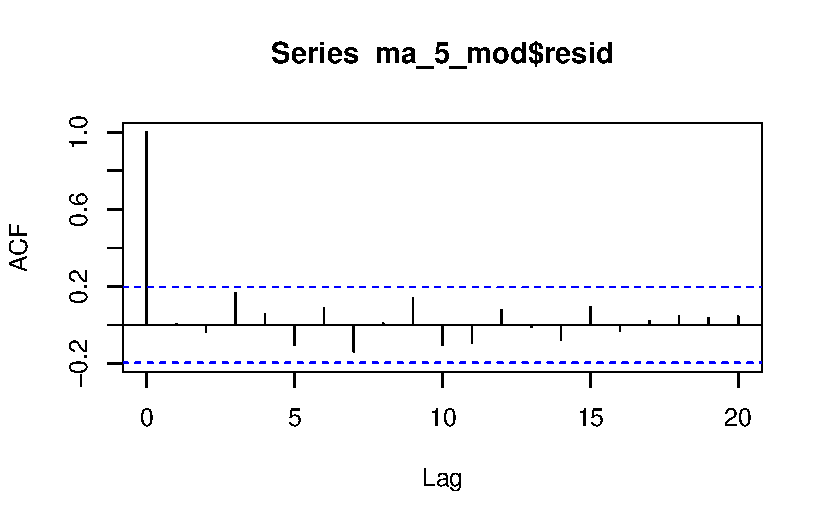
\includegraphics{Lecture7_files/figure-pdf/unnamed-chunk-24-1.pdf}

\begin{itemize}
\tightlist
\item
  Estimation procedure matters!
\end{itemize}

\subsection{A bit about the Nile Data}\label{a-bit-about-the-nile-data}

\begin{Shaded}
\begin{Highlighting}[]
\FunctionTok{tsplot}\NormalTok{(Nile, }\AttributeTok{xlab =} \StringTok{"Year"}\NormalTok{, }\AttributeTok{ylab =} \StringTok{"Discharge at Aswan, 10\^{}8 m\^{}3"}\NormalTok{, }\AttributeTok{main =} \StringTok{"Annual Volume"}\NormalTok{)}
\end{Highlighting}
\end{Shaded}

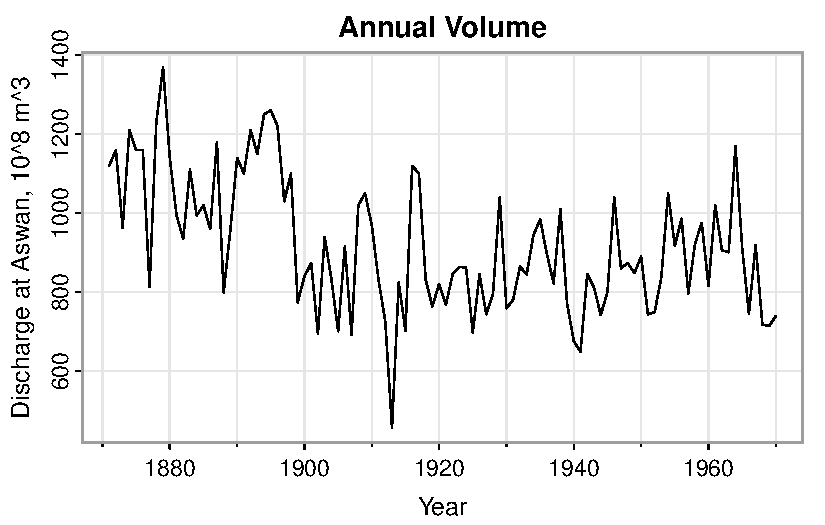
\includegraphics{Lecture7_files/figure-pdf/unnamed-chunk-25-1.pdf}

\subsection{Where's Aswan?}\label{wheres-aswan}

Sun directly overhead at noon on the summer solstice-- where the
circumference of the earth was calculated like 2000 years ago. So
cool!!! (not related to this data set(?))

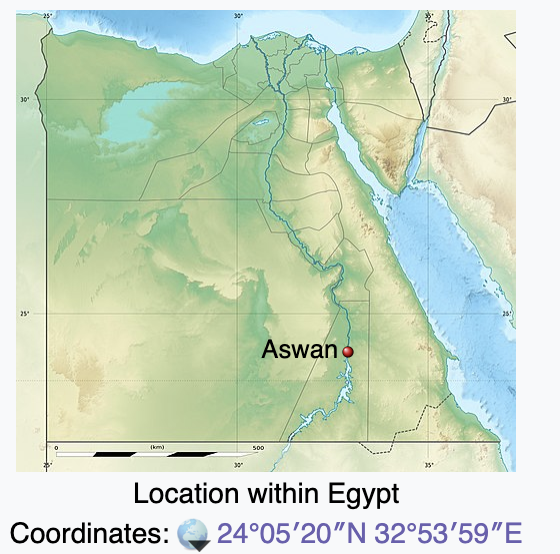
\includegraphics{images/Egypt map.png}

\subsection{A bit about the Nile
Data}\label{a-bit-about-the-nile-data-1}

``Level shift visible in the data at 1898'' -- how do we model ``abrupt
changes in distribution''?

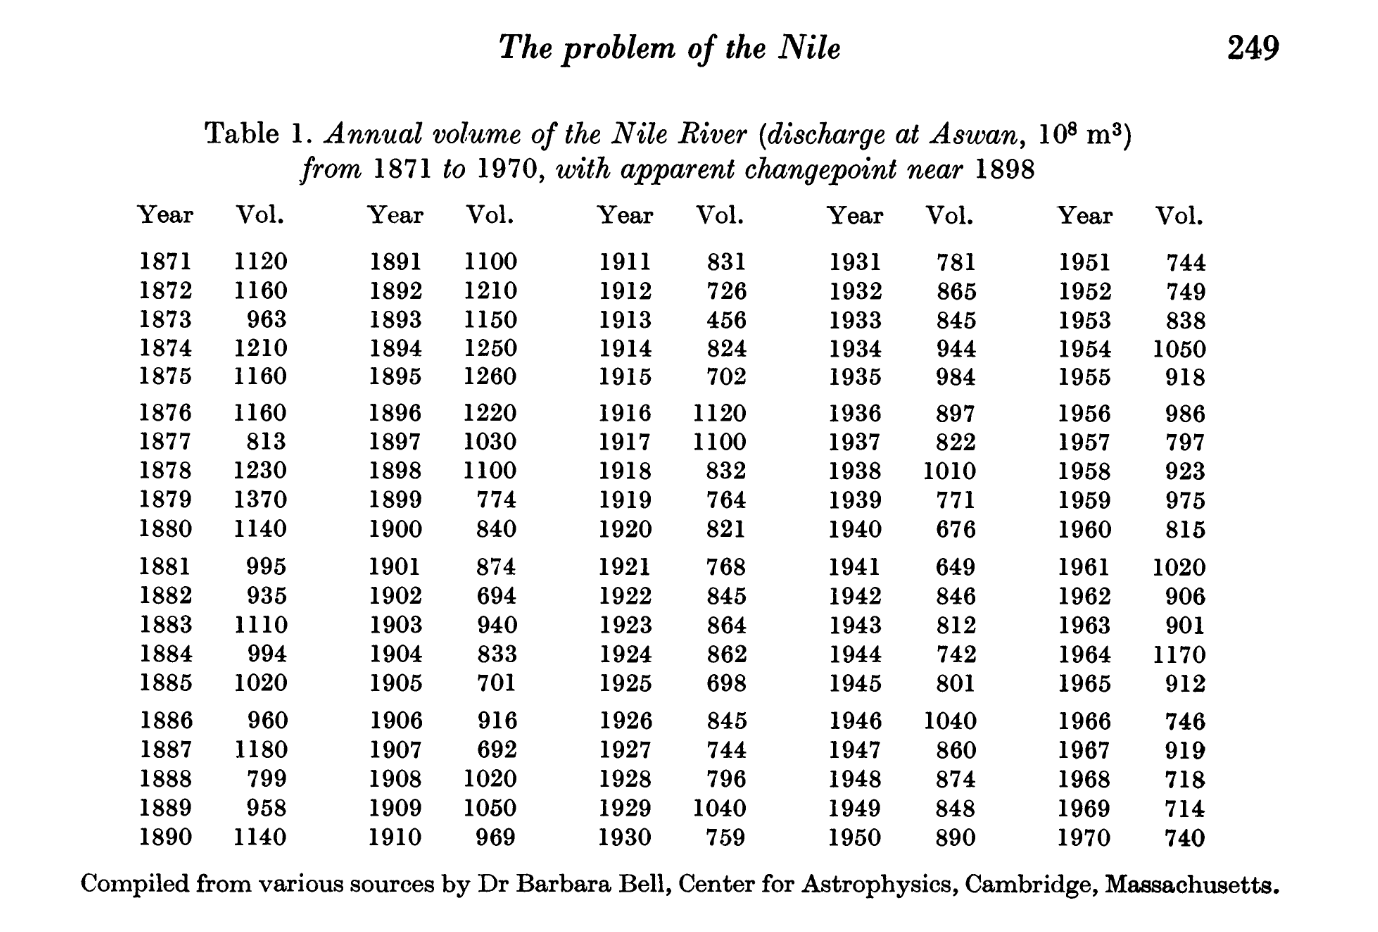
\includegraphics{images/table.png}

\subsection{Check out the paper!}\label{check-out-the-paper}

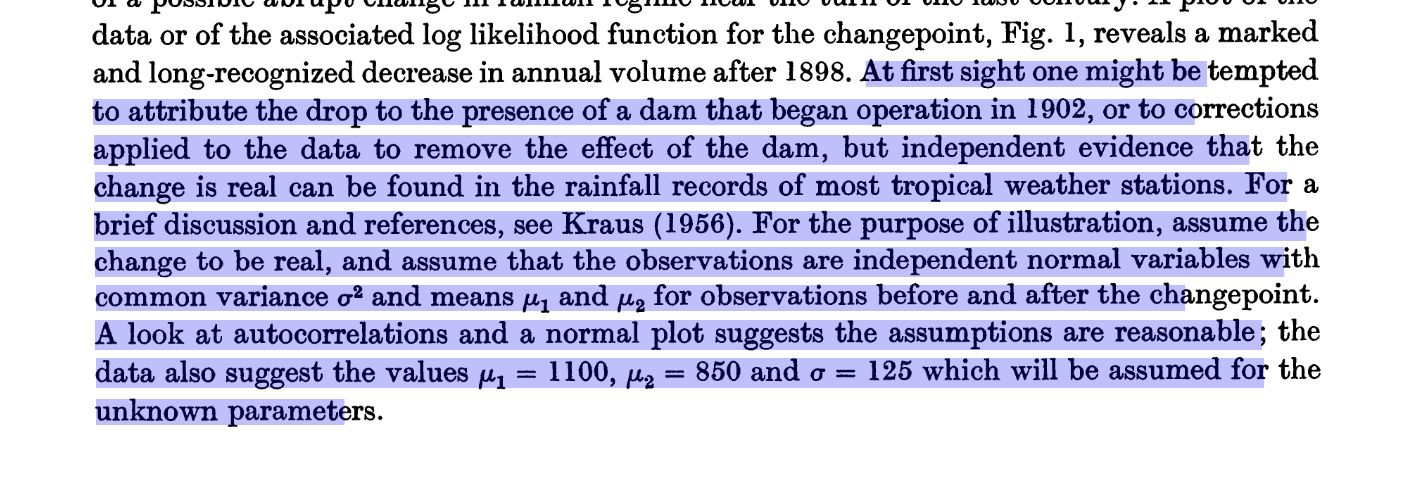
\includegraphics{images/early_time_series.png}

\subsection{Who's Barbara Bell?}\label{whos-barbara-bell}

She's not cited formally\ldots{} (data sets now get their own DOIs,
ideally)

\begin{itemize}
\item
  Got her PhD at Harvard in 1944 in Astrophysics

  \begin{itemize}
  \tightlist
  \item
    \href{https://www.radcliffe.harvard.edu/event/2012-its-complicated-exhibition\#:~:text=Mary\%20Whiton\%20Calkins\%20(Smith\%20AB,1886\%2C\%201890\%E2\%80\%931891).}{History
    of women at Harvard/Radcliffe} (a bit of a bummer to read)
  \end{itemize}
\end{itemize}

From (one of) her Obituary(ies):

``Working with Donald Menzel, Harold Glazer, Giancarlo Noci and Robert
Kurucz, \textbf{her research dealt primarily with observations of solar
phenomena}. Barbara had a keen interest in history and travel, and in
her later years traveled to all corners of the globe. She developed a
particular interest in the ancient history of Egypt. \textbf{Her
research expanded to include the variations in the floods of the Nile
for which she sought to connect to solar fluctuations}. Using ancient
accounts, she was \textbf{first to propose a linkage between prolonged
drought and the societal collapse she called ''The First Dark Age in
Egypt''} in the early 1970s. She published several journal articles on
the connection of climate fluctuations to the fall of Egyptian dynasties
which have been widely cited in the literature. Loved by all who knew
her, Barbara had \textbf{a sharp and curious mind, a kind heart and a
cheerful disposition}. Intensely interested in her family and those
around her, she donated generously her entire life to Harvard University
and numerous charities. A \textbf{beloved sister and aunt}\ldots{}''



\end{document}
